\section{Methodology \& Analyses}
Next to the data and the master data frame I explained in the previous data section, for this assignment I used a public GitHub repository \cite{GIT1} to store my documentation, images, notebook and report connected to this assignment. Everything was developed and programmed locally on my Macbook pro in a Python 3 / Anaconda setup and committed to the repository with the GitHub desktop client for OSX \cite{GIT2}. I used the regular Python libraries used in many data science assignments like \texttt{[pandas]} for handling data frames and \texttt{[requests]} for handling data retrieval via URL requests. For charting and graphics I used a combination of the \texttt{[matplotlib]} and \texttt{[seaborn]} libraries.
\\\\
Finding correlations can be easy if you have the master data frame well prepared. The \texttt{[analyses data frame]} as shown in the data section (see figure \ref{resultset}) only uses one line of code to come up with the correlation matrix. Both the input (\texttt{analyses data frame}) and the output (\texttt{correlation matrix}) are in the images below:
\\
\medskip
\begin{figure}[H]
	\begin{subfigure}{0.5\textwidth}
		\centering
		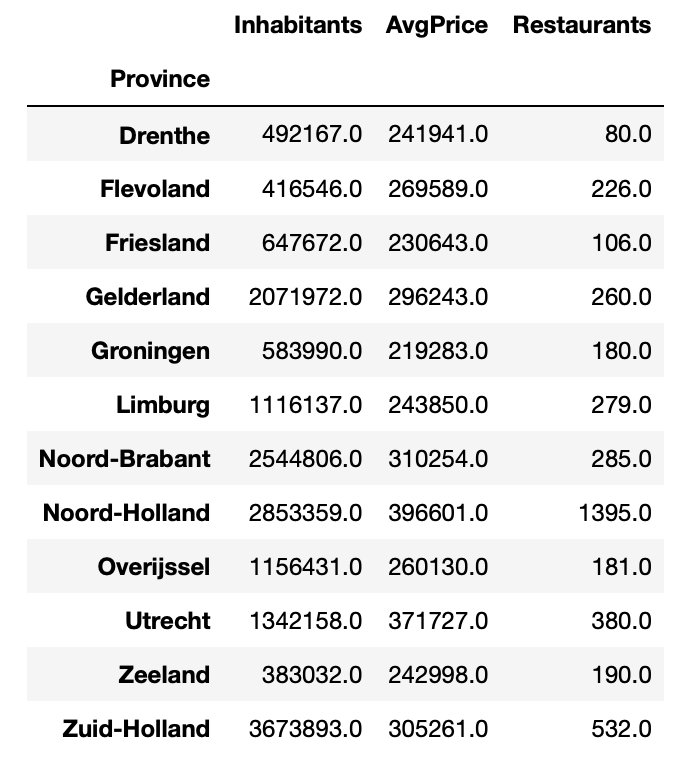
\includegraphics[scale=.4]{AnalysesSet} 
		\caption{}
	\end{subfigure}
	\begin{subfigure}{0.5\textwidth}
		\centering
		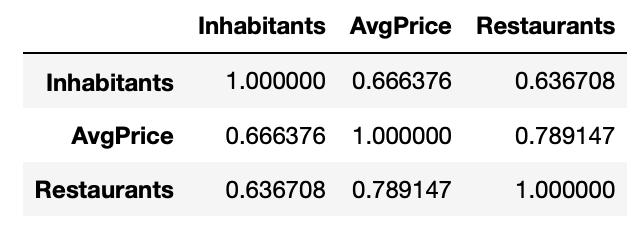
\includegraphics[scale=.4]{CorrMatrix}
		\caption{}
		\label{corMatrix}
	\end{subfigure}
\caption{Analysis data frame and calculates correlation matrix}
\end{figure}
\medskip
Based on the calculated correlation coefficients, I was able to do the analysis and come up with the desired results, which I compared to the rule of thumb mentioned on ResearchGate \cite{ART1} about the value of correlation coefficients. The IBM Data Science Professional course on Coursera covers a lot of model training and learning modules and during the course I had plenty of opportunity to play around with most modern types of analysis and machine learning techniques. The question underlying this report however, doesn't need a lot of computer calculation power to solve. Basically the methodology followed to answer the challenge summarises as follows:
\medskip
\begin{enumerate}
	\item Get the venues data from FourSquare
	\item Get the demographic data from CBS
	\item Get the price data from CBS
	\item Get the geo data from Arcgis
	\item Combine \& clean the data into a result set
	\item Use the correlation calculation of Pandas to calculate the correlation coefficients
	\item Analyse the results
	\item Plot the results on a map of the Netherlands
\end{enumerate}
\medskip
